% Generated by scripts/build_m3_paper_comparison.py; final common judge only.
\begin{table}[htbp]\centering\small
\caption{已完成配对子集的逐视频自动评分。保留全部97题；失败计零。}
\label{tab:videos}\begin{tabular}{lrrrr}\toprule
视频 & 题数 & oGMemory & M3-Agent & 分差\\\midrule
\code{study_09} & 12 & 0.5833 & 0.5000 & +0.0833\\
\code{kitchen_01} & 13 & 0.3846 & 0.1923 & +0.1923\\
\code{bedroom_05} & 12 & 0.4167 & 0.3750 & +0.0417\\
\code{study_23} & 14 & 0.6786 & 0.3214 & +0.3571\\
\code{kitchen_23} & 12 & 0.5417 & 0.6250 & -0.0833\\
\code{study_05} & 12 & 0.4583 & 0.3750 & +0.0833\\
\code{gym_03} & 11 & 0.7273 & 0.7273 & +0.0000\\
\code{bedroom_04} & 11 & 0.8182 & 0.4545 & +0.3636\\
\midrule
题目加权合计 & 97 & 0.5722 & 0.4381 & +0.1340\\
\bottomrule\end{tabular}\end{table}
\begin{figure}[htbp]\centering
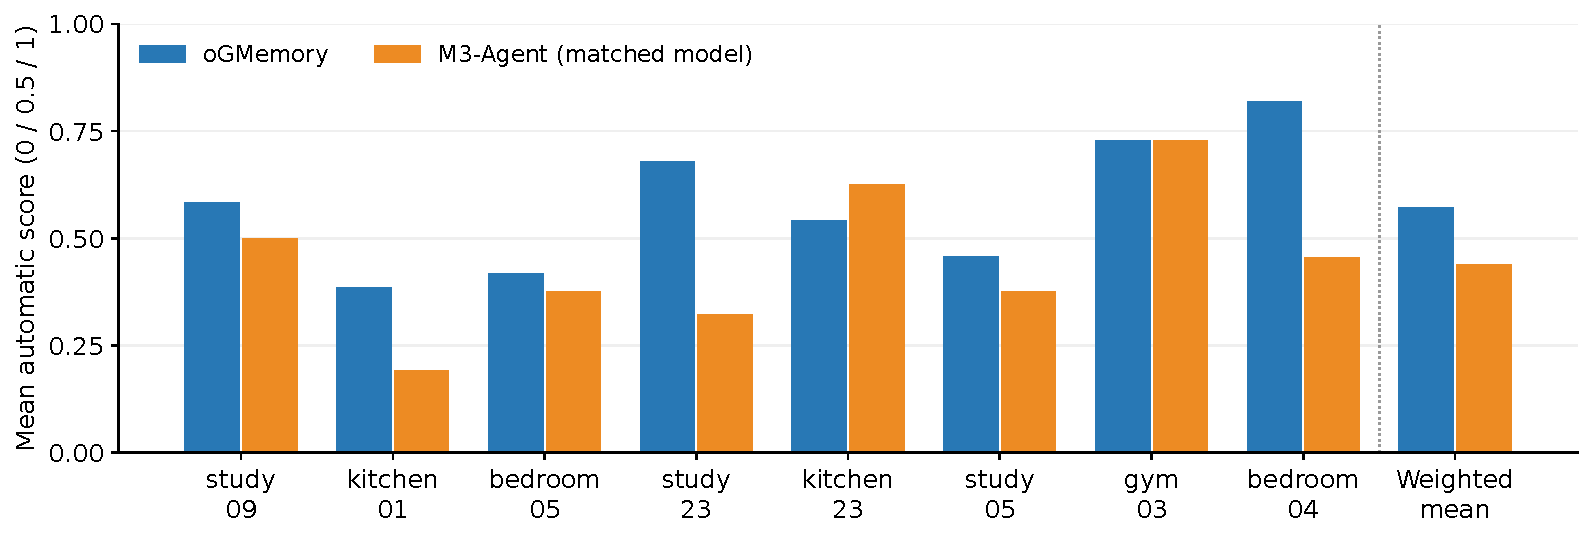
\includegraphics[width=\linewidth]{figures/paired8_final_scores.pdf}
\caption{两方法逐视频表现及题目加权均值。纵轴为自动评分而非人工准确率；不拼接早期临时评分或重跑答案。}\label{fig:scores}\end{figure}
\begin{table}[htbp]\centering\small
\caption{同一八视频子集的质量与资源开销。M为百万token，时间单位为分钟。}
\label{tab:resources}\begin{tabular}{lrr}\toprule
指标 & oGMemory & M3-Agent\\\midrule
有效回答 & 95/97 & 97/97\\
全分题比例（\%） & 51.55 & 37.11\\
QA输入（M） & 4.039 & 0.734\\
其中未缓存输入（M） & 2.129 & 0.263\\
QA输出，含推理（M） & 0.112 & 0.045\\
已记录建忆+QA总token（M） & 7.446 & 4.399$^{*}$\\
共享感知与启动 & 49.02 & 49.02\\
记忆、图谱及索引 & 573.46 & 249.64\\
QA耗时 & 65.91 & 31.02\\
各自计入感知后的总时间 & 688.39 & 329.68\\
\bottomrule\end{tabular}
\par\smallskip\footnotesize $^{*}$M3建忆有1次失败请求未返回usage，该总量仅表示已记录用量，不把未知值当作零；两方法QA用量完整。
\end{table}
\begin{figure}[htbp]\centering
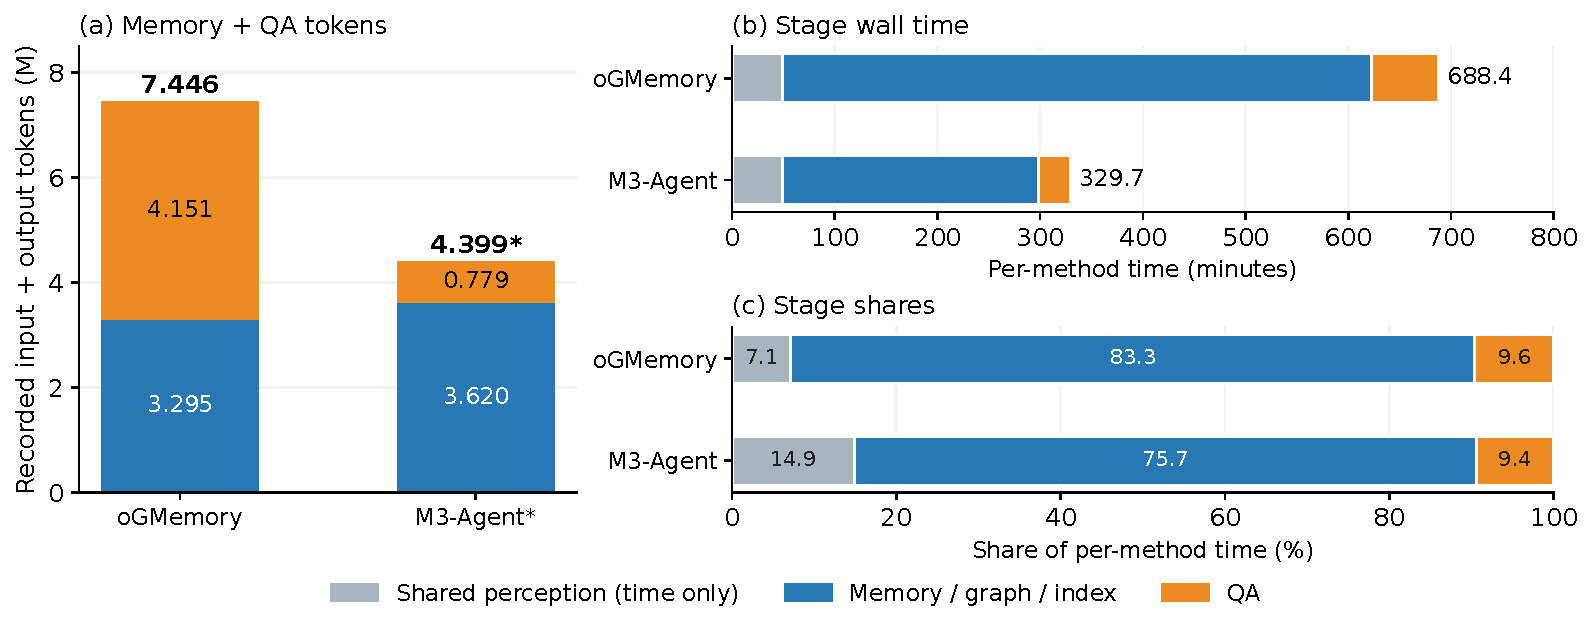
\includegraphics[width=\linewidth]{figures/paired8_final_resources.pdf}
\caption{资源开销及阶段分布。左图为建忆与QA已记录的输入、输出总token，不含embedding和评委；星号表示M3有未知建忆用量。右图将同一次共享感知分别计入两条方法路径；占比由累计耗时计算，不能将两方法总时间相加当作实验墙钟时间。}\label{fig:resources}\end{figure}
